

%  No need for this... space issues
% \begin{figure}
%     \centering
%     \resizebox{0.7\linewidth}{!}{\includegraphics{plots/Hyllus-architecture.pdf}}
%     \caption{Architecture (placeholder).}
%     \label{fig:arch}
% \end{figure}

% As shown on Figure~\ref{fig:arch},



\subsection{Limitations of Programmable Dataplanes}
While dataplane programming promises easy reconfiguration of network devices, it poses some challenges.
First, network devices support only a limited set of operations and control flows (no loops) without use of platform-specific \texttt{extern}s, and restrict the user to specific primitive data types, \ie, no floating-point units due to tight hardware constraints.
Second, these devices have limited low-latency memory (on the order of a few tens of \si{\mega\byte}s~\parencite{DBLP:conf/sosp/JinLZSLFKS17}) and do not provide dynamic memory management.
These limitations prohibit complex algorithms from being implemented, but allow certain restricted solutions, such as what is presented in DAPPER~\parencite{DBLP:conf/sosr/GhasemiBR17}, where the authors implement a TCP state machine purely in the dataplane.

\subsection{Histogram Generation}

\begin{figure}
    \centering
    \resizebox{\linewidth}{!}{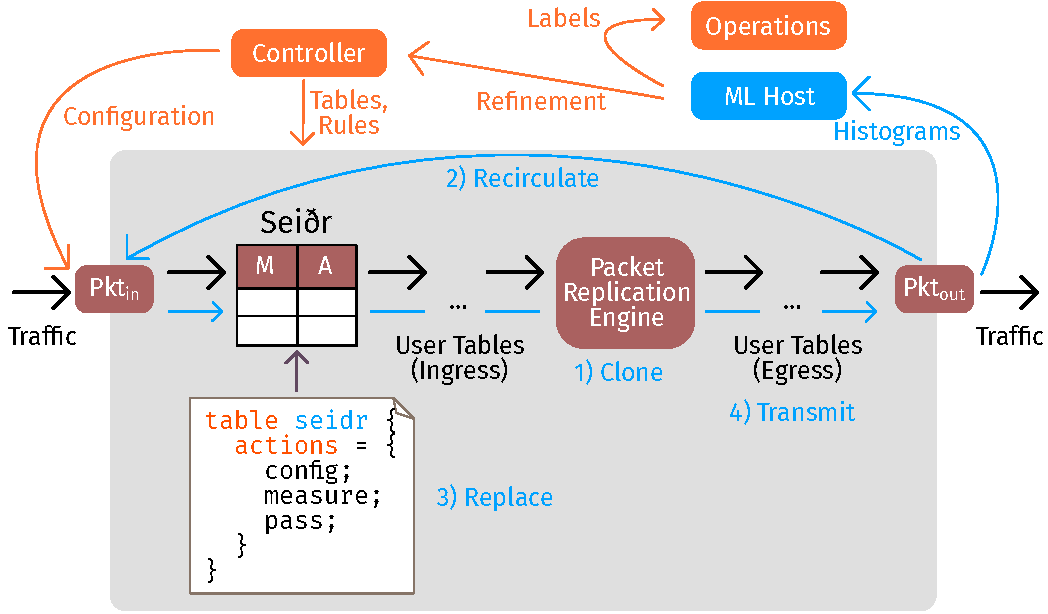
\includegraphics{diagrams/seidr/dp-arch-diagram.pdf}}
    \caption[\seidr{}'s integration with a PSA-compatible dataplane.]{\seidr{}'s integration with a \gls{acr:psa}-compatible dataplane. \seidr{} uses a register block to... When not using digests to emit packets... ?? must go through the above extended rigmarole}
    \label{fig:arch}
\end{figure}

% Let's show them a histogram datastructure would look like purely with registers and how would a P4 action populate it - pseudocode or P4 snippet would be nice.
\sidenote{?? FIGURE::: Can I redo this diagram to show the possibility of digest?}
Although packet timing information is useful in understanding network and flow behaviour, without volume or packet rate reduction it is prohibitively expensive for hosts to handle each packet.
Histogramming acts as the \emph{aggregation step} which makes this class of analysis feasible in high-speed networks.
\Cref{fig:arch} demonstrates how \seidr{}, installed as an additional table in any P4 program, records and transmits inter-arrival time histograms.
The format for these histogram packets is outlined in \cref{fig:seidr-headers}; we choose to store individual buckets as \mintinline{rust}{u16}s, and the number of buckets in any histogram is fixed at compile time.
We set this to \num{100} buckets per histogram.
Packets traverse a table which requires \num{3} actions to be implemented:
\begin{enumerate}
    \item \mintinline{rust}{config} reads any matched packets as a \mintinline{rust}{seidr_cfg_t} of type \mintinline{rust}{SET_}\{ \mintinline{rust}{MIN}, \mintinline{rust}{MAX}, \mintinline{rust}{DST}, \mintinline{rust}{SRC}, \mintinline{rust}{LEN} \} by using the P4 parser.
    These update registers \numrange{1}{5} in \cref{tab:registers}, dropping any matched packets.
    
    \item \mintinline{rust}{measure} calculates the inter-arrival time, update per-flow histograms, and transmits finished histograms to the correct host. We describe its operation in \cref{alg:measure}.
    
    \item \mintinline{rust}{pass} ignores packets, and is the default action.
\end{enumerate}
Constructing \seidr{} in this manner allows the control plane to install rules to enable/disable runtime reconfiguration as needed, and to monitor as many or as few flows as desired (\ie, using wildcard rules, or exact matching).

The PSA does not have any mechanisms for generating new packets.
To circumvent this, any packet which would complete a histogram is tagged for cloning at the end of the ingress pipeline, and recirculation at egress (\cref{algline:recirc}).
This truncated copy returns to \seidr{}'s table, where we enable the relevant headers, change L2/3 fields, and write out the histogram contents (\crefrange{algline:rewrite-start}{algline:rewrite-end}).
The P4 deparser outputs the new protocol stack at egress, and transmits the histogram UDP packet into the network.
Event-driven architecture proposals~\parencite{DBLP:conf/hotnets/IbanezABM19} may allow a more natural means of packet generation.

\begin{figure}
\centering
\begin{subfigure}{0.45\linewidth}
\centering
\adjustbox{max width = 0.6\linewidth}{
\begin{minipage}{\linewidth}
\begin{minted}[escapeinside=||]{rust}
|\textbf{\textcolor{Keyword}{header}}| seidr_cfg_t {
    bit<8> function;
    bit<144> payload;
}
\end{minted}
\end{minipage}
}
\end{subfigure}
\begin{subfigure}{0.45\linewidth}
\centering
\adjustbox{max width = 0.6\linewidth}{
\begin{minipage}{\linewidth}
\begin{minted}[escapeinside=||]{rust}
|\textbf{\textcolor{Keyword}{header}}| seidr_t {
    bit<128> src_ip;
    bit<128> dst_ip;
    bit<16> src_port;
    bit<16> dst_port;
    bit<16> eth_type;
    bit<BUCKETS * 16> histo;
}
\end{minted}
\end{minipage}
}
\end{subfigure}
\caption{P4 headers for \seidr{} configuration and histograms.}\label{fig:seidr-headers}
\end{figure}

\begin{algorithm}
% \vspace{-0.25cm}
% \DontPrintSemicolon
\KwData{5-tuple, P4 metadata, P4 headers, Registers}
h $\leftarrow$ hash(5-tuple)\;
index $\leftarrow$ BUCKETS * h\;
owner $\leftarrow$ HistoOwner[h]\;
\uIf{metadata.packet\_path = RECIRCULATE}{
    headers.tcp.valid $\leftarrow$ false\label{algline:rewrite-start}\;
    headers.udp.valid $\leftarrow$ true\;
    headers.seidr.valid $\leftarrow$ true\;
    copy 5-tuple into headers.seidr\;
    rewrite headers.ip, headers.udp using HistoSrc/Dest\;
    headers.seidr.histo $\leftarrow$ HistoData[index..]\;
    truncate payload\;
    zero out registers: BucketCount, HistoOwner[h], HistoData[index..]\;\label{algline:rewrite-end}
}
\ElseIf{owner = 0 \textbf{or} owner = 5-tuple}{\label{algline:owner-check}
    HistoOwner[h] $\leftarrow$ 5-tuple\;
    iat $\leftarrow$ LastTimestamp - metadata.mac\_ingress\_time\;
    \If{iat $\ge$ Min \textbf{and} iat $\le$ Max}{
        bucket $\leftarrow$ BUCKETS * (iat - Min) / (Max - Min)\;
        HistoData[index + bucket] $\leftarrow$ HistoData[index + bucket] + 1\;
        BucketCount[h] $\leftarrow$ BucketCount[h] + 1\;
        \If{BucketCount[h] = Len}{
            mark packet for cloning and recirculation\label{algline:recirc}\;
        }
    }
}

\caption{Histogram update and transmission.}\label{alg:measure}
\end{algorithm}

In the event of hash collision (\cref{algline:owner-check}), we ignore packets outside of the tracked flow to ensure that data is accurate.
As later processing and classification directly affect what decisions are made by operators or automatically taken by a policy (possibly leading to incorrect flow limits, QoS, \emph{etc.}), avoiding corruption/cross-contamination of operational data is paramount.
To gain collision resistance, Robin Hood hashing could be used up to a maximum distance in the table, treating a zeroed owner as empty and an illegal source IP as a tombstone value.

\begin{table}
    \centering
    \caption{Register map (Datatype, Amount) for an $h$-bit hash.}
    \resizebox{\linewidth}{!}{\begin{tabular}{@{}ccccccccc@{}}\toprule
        Min & Max & Length & HistoSrc & HistoDest & BucketCount & LastTimestamp & HistoOwner & HistoData \\ \midrule
        \mintinline{rust}{u16} & \mintinline{rust}{u16} & \mintinline{rust}{u16} & \mintinline{rust}{u16 + u128} & \mintinline{rust}{u16 + u128} & \mintinline{rust}{u16} & \mintinline{rust}{u64} & \mintinline{rust}{3 * u16 + 2 * u128} & \mintinline{rust}{BUCKETS * u16} \\
        1 & 1 & 1 & 1 & 1 & $2^h$ & $2^h$ & $2^h$ & $2^h$ \\ \bottomrule
    \end{tabular}}
    \label{tab:registers}
\end{table}

% Basic Logic:
% \begin{itemize}
%     \item table 1: three actions
%     \begin{itemize}
%         \item config: set R1 or R2 (controller installs rule matching a specific port/ip combo)
%         \item measure: take ingress timestamp from metadata, do stuff, write into lasttime, add to bucket and total if within bounds
%         \item pass (default)
%     \end{itemize}
%     \item then pass onto rest of tables
%     \item Why do it this way? can make it all or nothing through control plane.
%     \item How to write and send packet? Same trick as ESNET? (recirc w/ custom metadata to transform pkt)
% \end{itemize}

% ?? NOTE: See PSA \cite{p4-psa} for register format. Some papers, like Dapper, suggest that hash tables should be possible? That would work out very well in our benefit.

% ?? What is configurable? Min, max of the histogramming range

This design allows runtime configuration of all aspects save for the bucket count; at runtime, the only way to increase bucket resolution is to examine a smaller region of IATs.
While in theory this could be configured below a maximum compiled into the firmware, the difficulties introduced in classification/data processing make this infeasible.
Unless using stream-capable classifiers such as LSTMs~\parencite{DBLP:journals/neco/HochreiterS97}, changing the input size requires retraining from scratch since new neuron weights must be added and structural properties of the input data change.
Increasing the bucket count requires new firmware installation, as many dataplane P4 implementations cannot allocate variable-length stores due to the lack of a dynamic allocator.

\begin{figure}[t]
    \centering
    \begin{subfigure}[t]{0.49\linewidth}
        \centering
        \resizebox{\linewidth}{!}{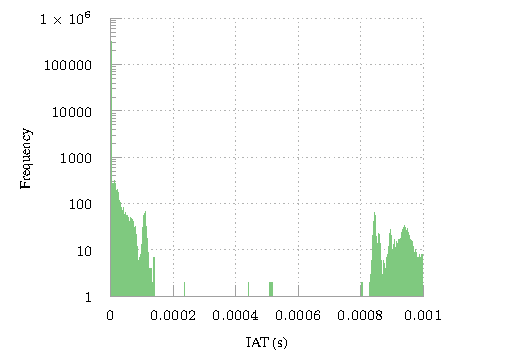
\includegraphics{plots/seidr/dt-cubic-1000-app.pdf}}
        \subcaption{TCP Cubic}
        \label{fig:cubic-hist-app}
    \end{subfigure}
    \begin{subfigure}[t]{0.49\linewidth}
        \centering
        \resizebox{\linewidth}{!}{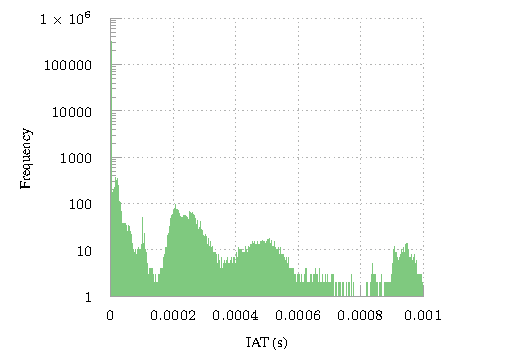
\includegraphics{plots/seidr/dt-bbr-1000-app.pdf}}
        \subcaption{TCP BBR}
        \label{fig:bbr-hist-app}
    \end{subfigure}
    \caption{Example dataplane histograms showing visible differences in inter-arrival times of selected TCP flavours. Our ML solutions are trained to programmatically identify such differences.}
    \label{fig:tcp-hist-app}
\end{figure}

As an example of dataplane-generated histograms, \cref{fig:tcp-hist-app} shows the distribution of inter-arrival times between two TCP congestion control algorithms. The visible differences are programmatically identified using our ML algorithms.

\subsection{Accurate, Precise and High-Resolution Timestamping}

Precise timestamps are critical when detecting temporal properties of flow behaviour, such as microbursts or inferring flow congestion control algorithms.
It is especially important in high speed (\SI{100}{\giga\bit\per\second}) networks, where there can be as little as \SI{6.7}{\nano\second} between packets that need to be analysed.
With a Linux-based software solution (\eg, reading packets from a link with \emph{tcpdump}), the Linux kernel can only provide microsecond-level accuracy with precision in the order of \SI{100}{\micro\second}~\parencite{DBLP:conf/noms/KundelSBRK20}.
DPDK improves on this, increasing the accuracy to \SI{100}{\nano\second} in the best case~\parencite{DBLP:journals/ccr/PrimoracBA17}.
However, today's dataplane devices (\eg, Netronome SmartNICs, NetFPGA SUME) allow nanosecond-accurate timestamps to be retrieved from the \emph{Media Access Control} (MAC) modules with a precision of \SI{10}{\nano\second}~\parencite{DBLP:conf/noms/KundelSBRK20}, a timestamp property \seidr{} relies upon.

% Some platforms provide picosecond-level precision and many solutions allow time synchronisation between multiple devices using the IEEE 1588-2002 (Precision Time Protocol) standard.

